\section{起二维滤波作用的波场外推}
一个脉冲函数($\delta$函数)可由许多正弦谐波(或复指数函数)的叠加构制出来,这是傅
氏分析的主要思想之一。在时间序列的研究中,就是用这种方法构制滤波器的脉冲响应。在
空间函数的研究中,则用这种方法来形成一个物理点源。

把时间特性与空间特性合在一起,就可将傅氏分量解释为单频平面波,物理光学(以及
与它有关的反射地震学)就成了滤波理论的一种推广情形。我们在本节中将研究惠更斯二次震
源在傅氏空间中的数学形式,就波场的空间外推而言,它就是一种二维滤波。
\subsection{射线与波前}
\begin{figure}[H]
\centering
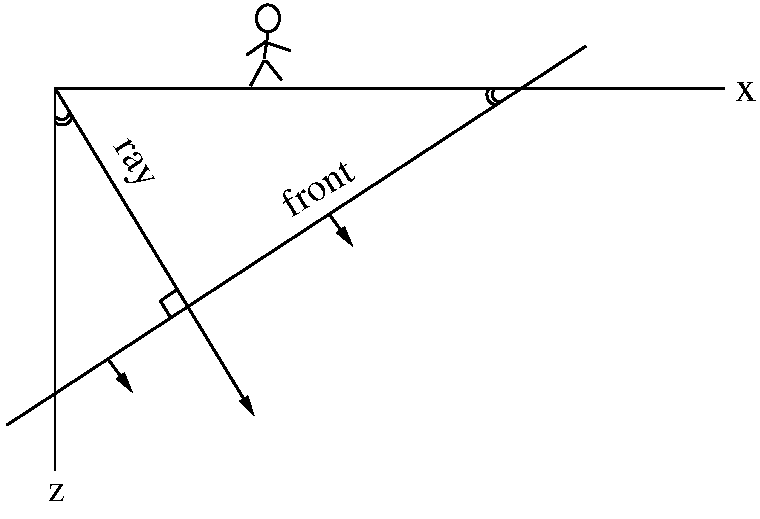
\includegraphics[width=0.5\textwidth]{omk/front}
\caption[front]{下行射线及其波阵面}
\label{fig:omk/front}
\end{figure}
  图\ref{fig:omk/front}所示是与垂直方向呈$\theta$角度向下移动进入地层的一个射线,垂直于该射线的是波
  阵面。根据基本的几何关系,波阵面与地表面之间的夹角也是。射线按速度$v$而增加其长度,在地表面上观察到的则是视速度,即波阵面与
  地面交点之移动速度,这种速度即为$v/sin\theta$,
  比速度$v$要快。类似地,波阵面与垂直轴之截
  点的速度(即垂直视速)为$v/cos\theta$。如图\ref{fig:omk/front}
  所示波阵面那样的直线,其数学表达式应为
  \begin{equation}
  z=z_{0}-xtan\theta
  \label{eq:ex1.2.1}
  \end{equation}
    在这表达式内,$z_{0}$是波阵面与垂直轴之间
    的截距.使该截点下行移动,用适当的速度乘以时间来代替它,则
  \begin{equation}
  z=v\frac{t}{cos\theta}-xtan\theta
  \label{eq:ex1.2.2}
  \end{equation}
    解出时间,得

  \begin{equation}
  t(x,z)=\frac{z}{v}cos\theta+\frac{x}{v}sin\theta
  \label{eq:ex1.2.3}
  \end{equation}

  式\ref{eq:ex1.2.3}可告诉我们关于波阵面通过任何特定位置$(x,z)$时的时间。对于任意形状具有时
  移的波形,其表达式以$f(t-t_{0})$表示。时移$t_{0}$用式\ref{eq:ex1.2.3}定义,可得出一个表示以某种
  波形沿射线移动的波场表达式

  \begin{equation}
  moving\ wavefield = f(t-\frac{z}{v}sin\theta-\frac{z}{v}cos\theta)
  \label{eq:ex1.2.4}
  \end{equation}

 \subsection{傅氏空间内的波}
 由正弦谐波的叠加,可构制出任意函数.经常出现的正弦谐波和复指数函数都是常系数
 线性偏微分方程的解,这就是它们出现的一个原因。之所以提到偏微分方程,是因为大多故
 物理定律都是可用偏微分方程表达的。


 对时间函数应用傅氏积另时,我们要遇到傅氏积分核$exp(-i\omega t)$。将式\ref{eq:ex1.2.4}中
 的任意函数具体化为函数$exp(-i\omega (t-t_{0}))$的实部,得

  \begin{equation}
  moving\ cosine\ wavefield = cos[\omega(\frac{x}{v}sin\theta+\frac{z}{v}cos\theta-t)]
  \label{eq:ex1.2.5}
  \end{equation}

  要把傅氏积分应用到空间坐标轴$x$必须定义空间圆频率。由于我们妓理问题时最终将会遇
  到大量空间坐标轴(炮点是三个坐标轴,检波点是三个坐标轴,中心点与炮检距也是三个坐标
  轴),所以就采用这样的约定:对字母$k$加一个下标示,用以表示对何种坐标进行傅氏变换.
  因此,$k_{x}$就是沿$x$坐标轴的空间圆频率,而$exp(+ik_{x}x)$则为其傅氏积分核。对每个坐标轴
  和傅氏积分核而言,还有一个$i$取什么符号的问题,此处采用大多数物理书籍中所采用的符
  号约定,即与式\ref{eq:ex1.2.5}
  所取符号一致的约定.如此选择的理由将在以后的\ref{subse:1.6}节中讨论。
  采用这种约定,波就是沿空间坐标的正方向移动,因而$(x,z,t)$空间的傅氏积分核将取
  为
  \begin{equation}
  Fourier\ kernel = 
                e^{ik_{x}x}e^{ik_{z}z}e^{-i\omega t} = exp[i(k_{x}x+k_{z}z-\omega t)]
  \label{eq:ex1.2.6}
  \end{equation}

  使式\ref{eq:ex1.2.5}
  等于式\ref{eq:ex1.2.6}
  的实部,可知角度与速度均与傅氏分量有关,应该牢记这些关系!

  \begin{equation}
  sin\theta=\frac{vk_{x}}{\omega},cos\theta=\frac{vk_{z}}{\omega}
  \label{eq:ex1.2.7}
  \end{equation}

  由此可导出具有同等重要性的关系,将上述角度定义代入熟悉的关系式$sin^{2}\theta+cos^{2}\theta=1$
  ,就得出以标量波动方程波散关系而知名的一项极重要关系

  \begin{equation}
  k^2_{x}+k^2_{z}=\frac{\omega^{2}}{v^{2}}
  \label{eq:ex1.2.8}
  \end{equation}

  我们以后将会遇到波散关系和标量波动方程.式\ref{eq:ex1.2.8}的重要性在于:它能使我们区
  出一个实际是波场的无序函数同一个任意函数之间的差别.对任何一种函数$p(t,x,z)$,进行傅氏变换
  使之变为$P(\omega,k_{x},k_{z})$,现在对$P$的
  任何非零值所相应的$(\omega,k_{x},k_{z})$体
  作一下考察.显然,当且仅当$P$的所有非零值具有可满足式\ref{eq:ex1.2.8}
  的坐标时,它才会是一种波场。更有甚者,在实际情形
  下,$z=0$依从关系则是未知的。于是,假定$P$是一个波场就可以求出关于$z$的依从关系,因而根据
  式\ref{eq:ex1.2.8}能就关于$z$的依从关系作出推断。
  
\subsection{偏移可改善水平分辨率}
在原理上,偏移就是将一些双曲线转换成一些点。在实际上,双曲线并不蜕化成点,它
们是蜕化成一个焦点。焦点具有可测度的大小尺度。说偏移效果“良好”,是因为它增加
了空间分辨率,它把一个很大的双曲线压缩成一个细小的焦点。为定量描述偏移改善分
辨率的作用,必须定双曲线的尺度和焦点的尺度。图\ref{fig:omk/fwidth}所示是测定
双曲线尺度的各种不同方法。
\begin{figure}[H]
\centering
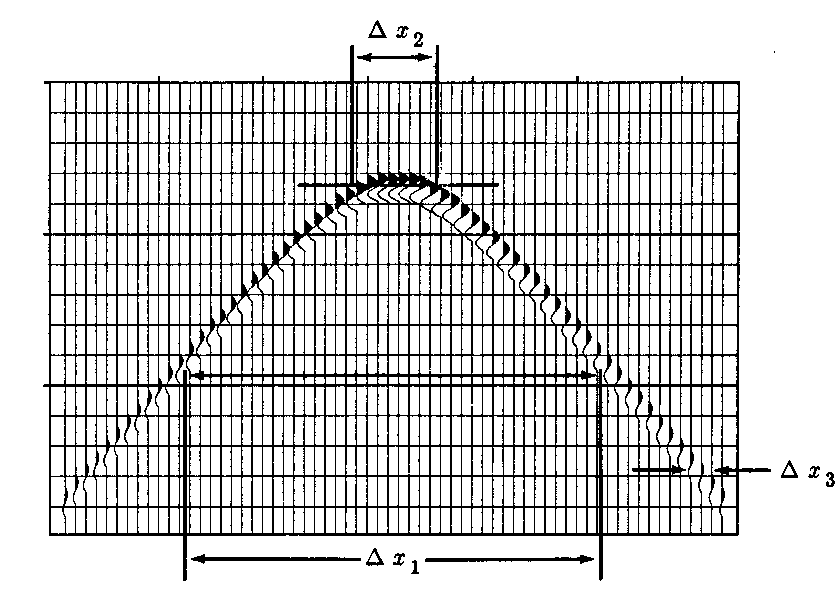
\includegraphics[width=0.6\textwidth]{omk/fwidth}
\caption[fwidth]{双曲线宽度参量的测定}
\label{fig:omk/fwidth}
\end{figure}
双曲线由地震脉冲组成,所以,根据主能量脉冲在时间轴上的各零交点之间的距离,可
租略大致估计双曲线的$\omega$频宽。典型的频宽值最50赫兹,不过你也可能遇到四倍
高一点或四倍低一点的值。决定深度分辨率的因素是关于地震波速度的知识,速度的典
型值为$3km/s$,不过你再一次可能会遇到四倍大一点或四倍小一点的速度。取这些值
意味着地震波长是实际波长的一半。之所以为一半,是由于在爆炸反射面计算中取了速度
$v$值的二分之一;或者与此等价,是由于将地震波长理解为被平分为上行部分与下行部分
了。习惯上,分辨率限定为有效波长的二分之一,或者大约为$15m$。地震分辨率是否应
取半波长$(15m)$或更小一些的值,这是个可以争论的问题,它涉及到关于信噪比的考虑,
超出了我们现在研究的范围。

横向分辨率需要估计双曲线宽度和焦点宽度。图\ref{fig:omk/fwidth}表示有三种双曲线
宽度定义,最宽的$\Delta x_{1}$大约包括双曲线四分之三的能量;其次是宽度$\Delta x_{2}$,
称作菲涅尔带(Fresnel Zone),它是初至正好改变极性时在两个时间上穿过双曲线的横截
距离。第三种是最小的可测宽度,位于远离双曲线顶部的侧翼上,这类宽度$\Delta x_{3}$
是所求出的最短水平方向波长。所谓分辨率就是误差范围大小的研究,所以,使误差本身
精确并没什么特别用处,主要知道$\Delta x_{1}>\Delta x_{2}>\Delta x_{3}$也就可以
了。空间波数$k_{x}$谱宽度大约为$1/\Delta x_{3}$。偏移究竟可以形成多么小的焦点呢
?这点将受到空间波数$k_{x}$谱中可达到的频宽所限制;焦点的范围大小将与$\Delta x_{3}$
大体相同。

图\ref{fig:omk/fresnel}是表示菲涅尔带概念的几何图形。菲涅尔带就是一个球面波与一
平面的相交截面、亦即球面波穿过该平面达到半波长深度时的截面。菲涅尔带宽度$\Delta x_{2}$
有什么意义呢?试想像你自己是在柏林市,那里有一堵“柏林墙”,你也许不被允许走近它。
假如墙上有一个洞,你现在向墙那一边的一位朋友大声打招呼。声音的响度是如何依赖于
墙洞的大小$\Delta X$呢?这并非明显易见,然而理论上和实验中众所周知的事实是:墙洞
比菲涅尔带大,就会引起声音稍微衰减,可是比较小的墙洞又会限制声音的传播,限制的
程度与该墙洞的大小成比例。
\begin{figure}[H]
\centering
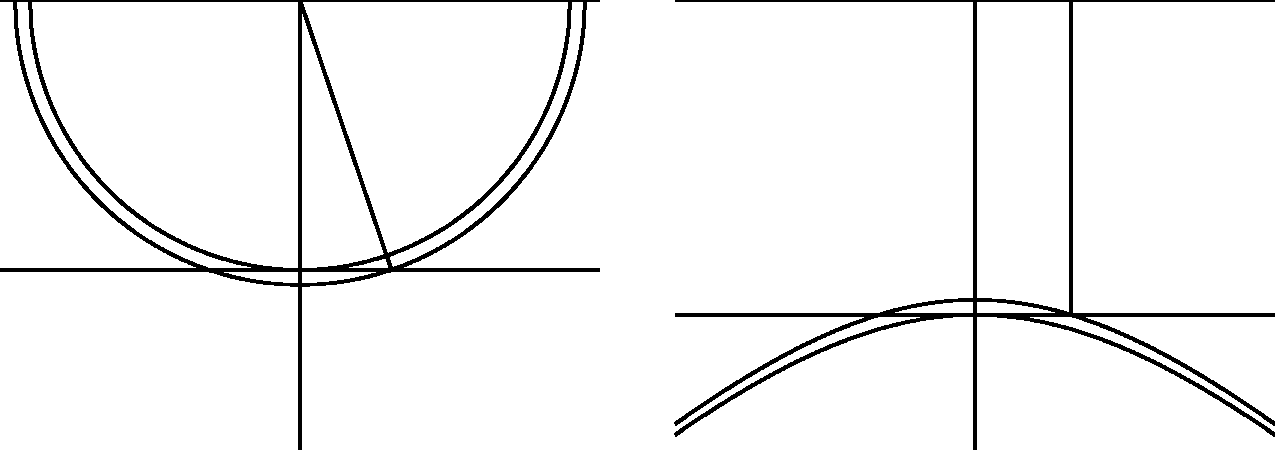
\includegraphics[width=0.95\textwidth]{omk/fresnel}
\caption[fresnel]{$(x,z)$空间内的菲涅尔带(左)及$(x,t)$空间内的菲涅尔带(右)}
\label{fig:omk/fresnel}
\end{figure}

波动传播相当于一种褶积滤波,从沿反射面分布的一个区域$\Delta x_{2}$(或地下一个
区域$\Delta x_{1}$)至地面上某一点这个范围内的信息,均受其影响。波动传播的逆过程
,即偏移,则相当于一种反褶积处理。横向分辨率的高低归根结底要查资料的空间频宽所限制。

即使是在反射面未表现出有倾角的地方可能还需有求于偏移。当要求必须在小于$\Delta x_{2}$
的精度范围之内来选定一个井位时,解释人员就得仔细检查振幅或波很沿反射面有何细微变化出现;
偏移使这些振幅变动与波形变动沿着反射面发生变化并有水平方向移动,所移动的距离就大约等于
菲涅尔带。

地震波速度随深度而增大是造成分辨率受限制的原因,这是反射地震学中的一项基本事实。由此
而出现:波越深地传播进入地层时,由于速度不断增大,它们的空间波长就越长。垂直分辨率
的情形简单说来就是这样:波长越长,分辨率就越低。水平分辨率的情形也类似,只不过水平
波长是在地表面上直接测定的。图\ref{fig:omk/hyp2}就是说明这种情形。图中所示是浅部散射
体和深部散射体形成的双曲面,浅部双曲线顶部到达时间早且有较陡渐近线,深部双曲线顶部到
达时间晚且有不太陡的渐近线。不太陡的渐近线有比比较长的水平波长,尽管速度随深度而增大,
地面上所测定的水平波长在同一深度并不改变(\ref{subse:1.5}节证明,这暗示着Snell定律)。
所以,横向空间分辨率随深度之増大而变坏。上述关于分辨率降低的原因综合起来,就可以解释
说明为什么在较晚的旅行时间上出现高频能量损耗。

\subsection{二维傅氏变换}
在更深入一步讨论之前,且先回顾一下关于二维傅氏变换的若干基本事实。二维函数在计算机
内以矩阵内的数值代表。计算机内的一维傅氏变换是一种向量运算。二维傅氏变换可以采用一
系列一维傅氏变换来进行计算,你可首先变换矩阵的每一列向量,然后再变换矩阵的每一行向
量:换一种办法,先进行行向量后进行列向量的变换也行。用图形表示如下:

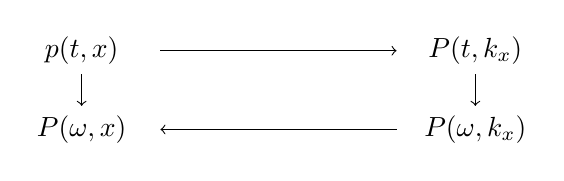
\begin{tikzpicture}
\draw[->] (11.0,1.5) -- (14,1.5);
\draw[<-] (11.0,0.5) -- (14,0.5);
\node at (10,0.5) {$P(\omega,x)$};
\node at (10,1.5) {$p(t,x)$};
\draw[->] (10,1.2) -- (10,0.8);
\draw[->] (15,1.2) -- (15,0.8);
\node at (15,0.5) {$P(\omega,k_{x})$};
\node at (15,1.5) {$P(t,k_{x})$};

\end{tikzpicture}

该图有个符号问题要注意,我们不能继续采用通常的符号约定:以小写字母代表物理空间
域,以大写字母代表傅氏变换域:因为那种约定不可能包括混合对象$P(t,k_{x})$和$P(\omega,x)$。
看来,与其是创造一些新符号,还不如最好是让读者利用该图所示上下关系去妥善处理这个
符号问题。函数的自变量必须有助于函数的命名,不要相混。

图\ref{fig:dft/plane4}所示是对典型的深海地震资料进行这些变换的一个例子。
\begin{figure}[H]
\centering
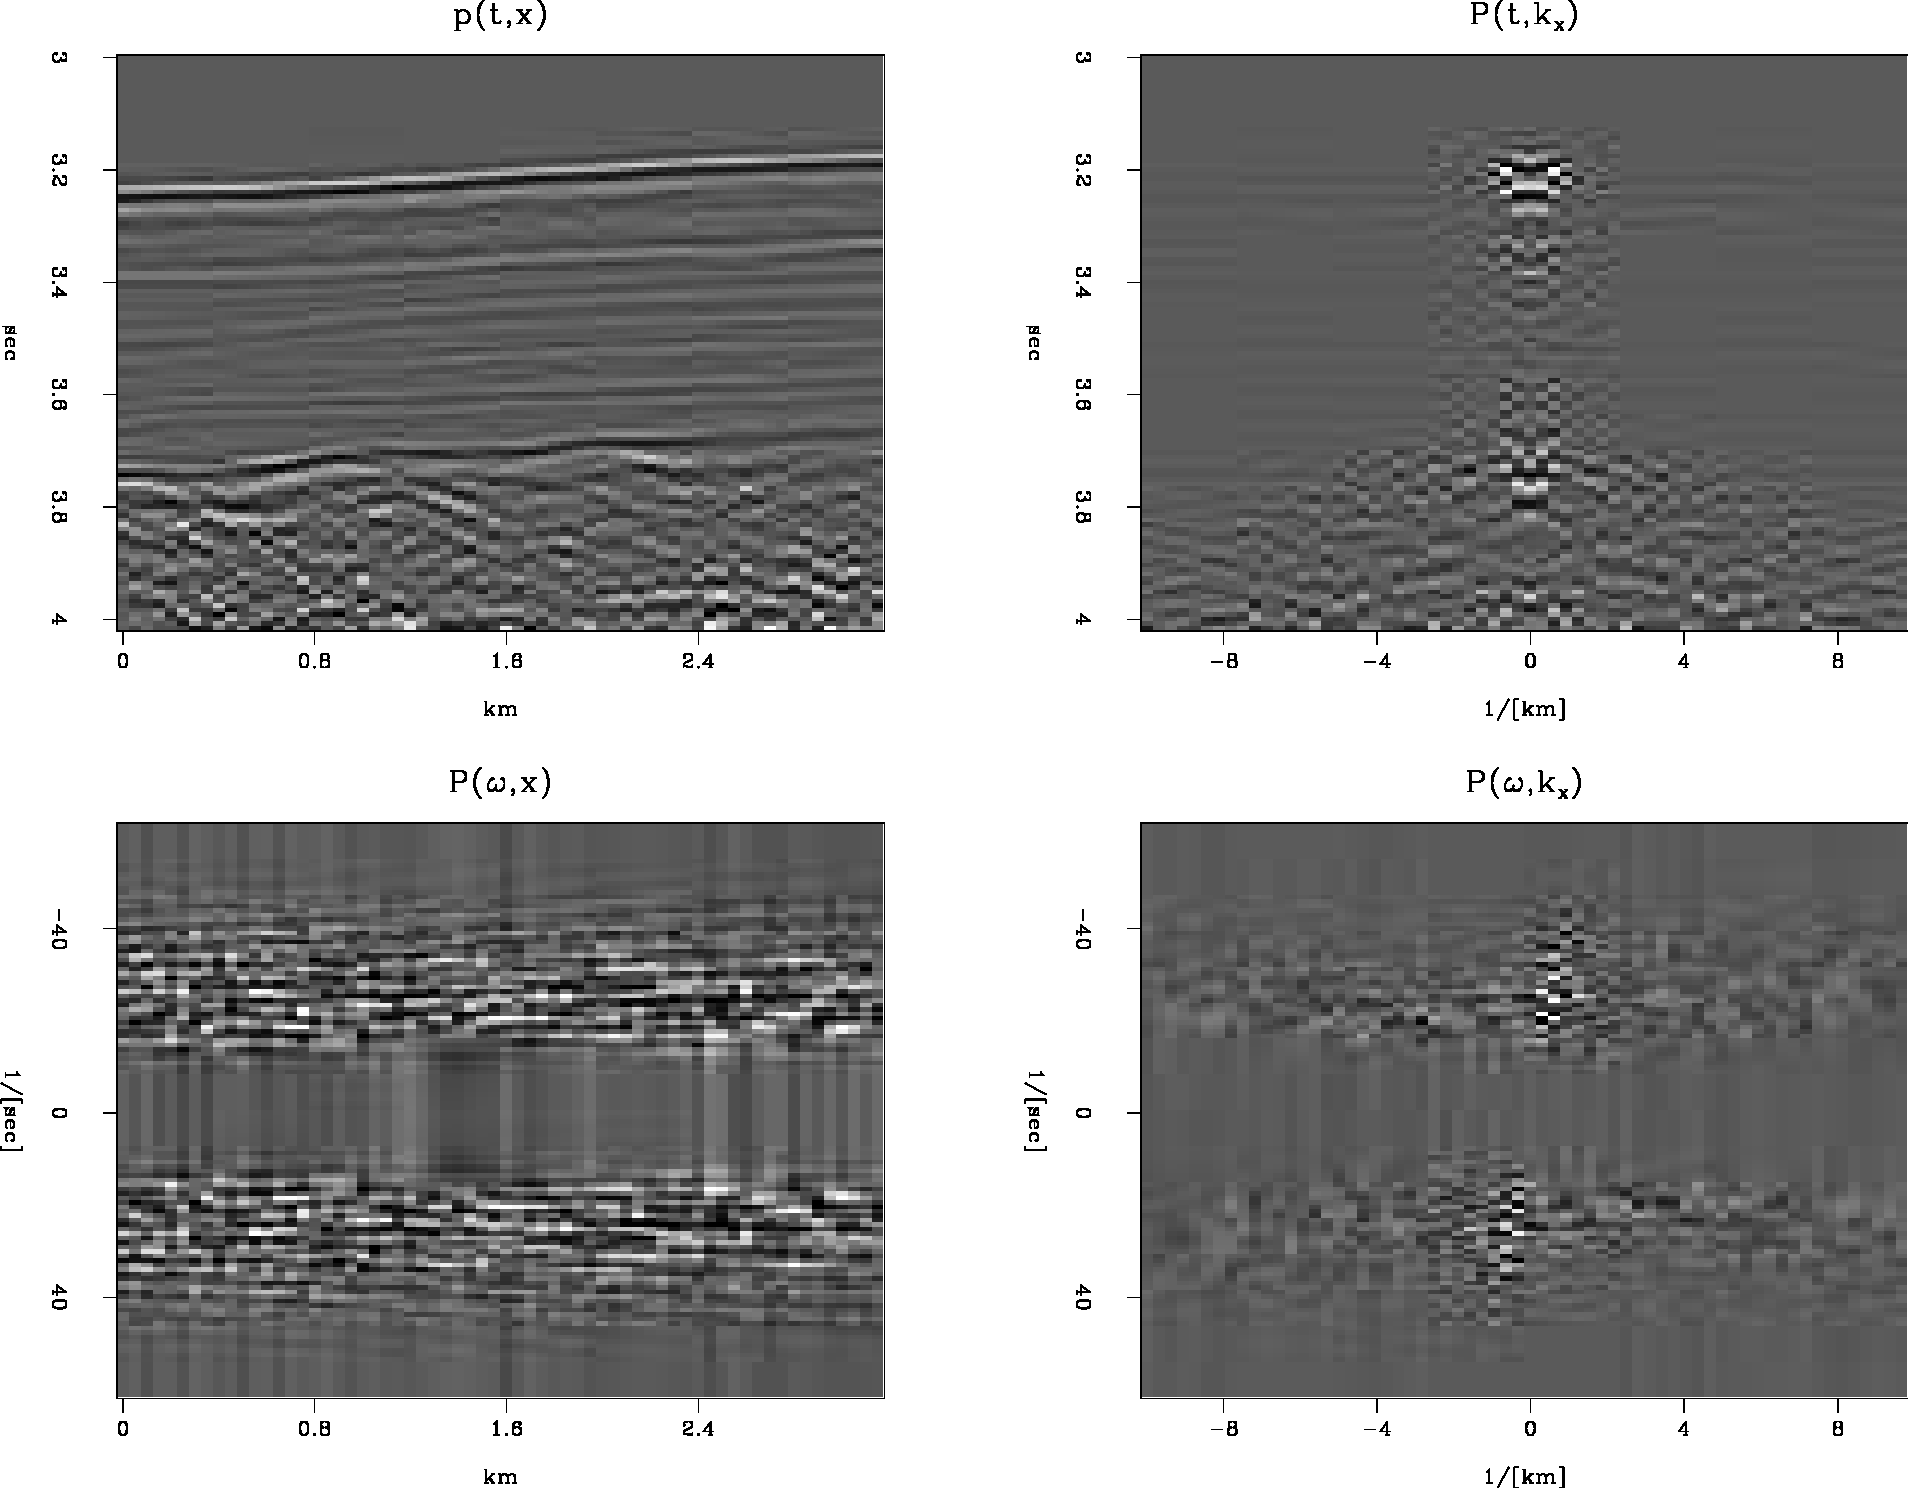
\includegraphics[width=0.95\textwidth]{dft/plane4}
\caption[plane4]{深海地震时间剖面$p(t,x)$及其各种傅氏变换的实部。由于通过水层
的旅行时太长,图中的时间轴未从$t=0$时开始}
\label{fig:dft/plane4}
\end{figure}

在深海,沉积物均属细粒并缓慢沉积为平缓而又规则的水平地层。缺少像砂岩那样的具
有渗透性的岩石,大大降低了从深海寻找石油的可能性。细粒页岩覆盖在不规则的基底
火成岩之上。在$P(t,k_{x})$的图中,低$k_{x}$值处有很强的谱,表示沉积地层具有横
向连续性;$k_{x}$的这种谱延伸至很大$k_{x}$值,致使深资料可能受到一点空间假频
影响(采样点过稀),这表示存在有火成岩。$P(\omega,x)$的图形表示该资料包含的不是
低频能量,能量在很大$\omega$时并不如所预料那样很快衰减,这表明存在有时间方面的
假频。在$p(t,x)$图形中,这种假频现象在阶梯状外形的海底初至中也是很明显的。倾斜
的海底在$(\omega,k_{x})$空间内表现为能量以某一种角度通过原点。

总而言之,一个地震记录集合的二维傅氏变换仅只涉及对每一地震记录进行两次一维傅
氏变换的计算,这是很幸运的事。为证实上述处理办法确实是实现二维傅氏变换,让我
们列出一些方程,首先说一下,任何$x$与$t$的函数均可表示为谐波函数之叠加和(傅
氏变换中采用的符号约定将在\ref{subse:1.6}节中解释),即
\begin{equation}
p(t,x) = \iint e^{-i\omega t+ik_{x}x}P(\omega,k_{x})d\omega dk_{x}
\label{eq:ex1.2.9}
\end{equation}
这种逆傅氏变换中的积分核具有波的形式——沿$x$轴的正方向传播的波。同样地,在正傅氏
变换中,为保持积分核是一个沿正方向传播的波,两个指数的符号均应改变。式中,为方便
起见,比例因子与无穷积分限均已略去。(离散计算时,积分限与比例因子均各不相同,何
必为此操心费事?)重积分可加括号,以表明要首先完成时间方面的变换
\begin{align*}
   & p(t,x) \notag \\
={}& \int e^{ik_{x}x}[\int e^{-i\omega t}P(\omega,k_{x})d\omega]dk_{x} \notag \\
={}& \int e^{ik_{x}x}P(t,k_{x})dk_{x} \notag
\end{align*}
括号内的量是就每个$k_{x}$完成的对$\omega$的傅氏变换。换一种方式也行,将$k_{x}$积分
放在括号内首先完成运算,那意味着首先完成行运算而不是列运算(或者反之)。正是函数$exp(-i\omega t+ik_{x}x)$
分离为两个指数之乘积的这种可分解性,才使进行这种重积分的计箅轻而易举而又节省时间。

\subsection{输入输出关系}
将数据资料向下延拓是偏移过程的核心部分。已知在地表面$z=0$这个平面上的输入数据,
我们必须构制出在深度$z$上可被记录到的数据。这点在傅氏变换域内很容易做到,这种
方法可被看作是直接乘以某个复指数的乘法运算,即
\begin{equation}
P(\omega,k_{x},z) = P(\omega,k_{x},0)e^{ik_{z}(\omega,k_{x})z}
\label{eq:ex1.2.10}
\end{equation}
既然运算是傅氏变换域内的一种乘法,那就能够用图解方式描述它:

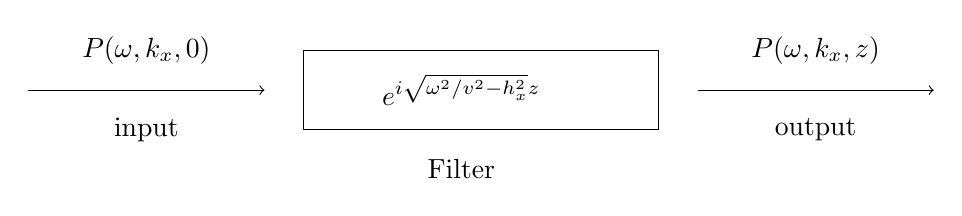
\begin{tikzpicture}
\centering
\draw[->] (2.0,1.5) -- (5.0,1.5);
\node at (3.5,2.0) {$P(\omega,k_{x},0)$};
\node at (3.5,1.0) {input};

\draw (5.5,1.0) rectangle(10,2.0);
\node at (7.5,1.5) {$e^{i\sqrt{\omega^{2}/v^{2}-h_{x}^{2}}z}$};
\node at (7.5,0.5) {Filter};

\draw[->] (10.5,1.5) -- (13.5,1.5);
\node at (12,2.0) {$P(\omega,k_{x},z)$};
\node at (12,1.0) {output};

\end{tikzpicture}

在频率$\omega$域内和波数$\k_{x}$域内,向下延拓都是一种乘积关系,那么该滤波器在
时间和空间域内看来又像是什么呢?原来它像是一神圆锥,粗略地说,这是$x^{2}+z^{2}-v^{2}t^{2}$
的一个脉冲函数;更精确地说,这是惠更斯二次波震源,前面曾经用海洋波浪通过防波堤
的一个空隙洞穴为例说明过它。将防波堤内多种多样空穴的响应相加起来,那就是遍及$x$
轴的褶积,将许多入射海波叠加起来,那就是遍及时间$t$的褶积。

现在让我们来看一下为何向下延拓滤波器会具有所述数学形式。$\omega,k_{x}$平面内的
每一点都与一正弦平面波有关,随深度而发生变化也将是正弦函数形式、即$exp(ik_{z}z)$,
对该正弦波而言,求解出方程$(8)$就可直接求出$k_{z}$的值:

\begin{subequations}\label{eq:ex1.2.11}
\begin{equation}
k_{z}=\pm(\frac{\omega^2}{v^2}-k_{x}^{2}) \label{eq:ex1.2.11a}
\end{equation}
\begin{equation}
 =\pm \frac{\omega}{v}(1-\frac{v^2k_{x}^{2}}{\omega^{2}})^{1/2} \label{eq:ex1.2.11b}
\end{equation}
\begin{equation}
 =\pm \frac{\omega}{v}cos\theta \label{eq:ex1.2.11c}
\end{equation}
\end{subequations}
选择正号意味着$exp(-i\omega t+ik_{z}z)$是一下行波(因为$z$随$t$之增大而增大时相位
将保持恒定);选择负号则形成一上行波。爆炸反射面概念要求有上行波,所以我们几乎总
是采用负号,不论我们是进行偏移还是进行摸拟。

取$e^{i\phi}$形式的输入输出滤波器看来是没有振幅比例因子的相移滤波器,这对我们计划进
行反褶积处理是一个好兆头,因为这意味着关于信噪比的顾虑,对于偏移处理要比对于普通
的滤波处理少得多了。

\subsection{习 题}
\begin{enumerate}
\item
    假设你能在普通地震频率范围内观测到某些横波,请问空间分辨率较之通常情形
是好一些、是一样、还是变坏了?为什么?
\item 
    试对本书中有关野外资料上的双曲线形初至浏览一下并测定其弗莱涅带宽度,在
没有零炮检距记录之处,有效的近似必须是沿一倾斜的直线测定${\Delta x_{2}}$
的大小。
\item
试对图\ref{fig:dft/plane4}中的$P(\omega,x)$图形内之水平“成层”现象作出解释。
该“层”之间距由什么决定?“层”的斜率由什么决定?
\item 
试问日本海槽有多深(水层速度为1.5公里/秒)?
\item 
    波场随时间的演交由下式描述
\begin{equation*}
p(x,z,t)=\iint[P(k_z,k_z,t=0)e^{-ix(k_x,k_z)}]e^{ik_xx+ik_zz}dk_xdk_x
\end{equation*}
设$P(k_x,k_z,0)$为常数,表示$(x,z)$空间中位于原点上的一个点源;令$t$非常大,意即被
积函数中的相位$\phi=[-\omega(k_x,k_z)+k_x(x/t)+k_z(z/t)]$是随$k_x$与$k_z$之变化而急
速改变。设仅当该相位为平稳相位时时,即$\partial\phi/\partial k_x$和$\partial\phi/\partial k_z$
均为零时,该相位才对积分有显著影响。试问同相轴位于$(x,z,t)$空间内何处?
\item 波场向下延拓以下式表示
\begin{equation*}
p(x,z,t)=\iint[P(k_z,z=0,\omega)e^{-ik_z(\omega,k_z)z}]e^{i\omega t+ik_xx}d\omega dk_x
\end{equation*}
设$P(k_x,0,\omega)$为常数,表示在空间内原点上的一个点源。试问同相轴应位于$(x,z,t)$
空间内何处?
\end{enumerate}
